\chapter{Introduction}
	\label{chap:intro}
	
	\section{Current State of Mobile Cyber Security}
		\label{sec:intro_motivation} 
		
		Ever since the release of the iPhone in 2007, smart phones and other mobile devices have played an increasingly larger role in our lives. We are using mobile devices for education, social interaction, commerce, mobile banking, entertainment, work, and more. 
		
		In the first world, mobile device usage has become ubiquitous. In the UK, smartphones became the most widely owned internet-enabled device in 2015 \cite{ofcom_coms_report}. Moreover, 52.6 percent of global web traffic came from mobile devices in 2019, up from 31.6 per cent in 2015 \cite{statista_mobile_web_traffic}. 
		
		Given the statistics from above, you would hope that mobile app developers have learned lessons from their desktop counterparts, and therefore, the majority of mobile apps are reasonably secure.
		
		That assertion proves to be false. A study done by cyber security consultancy Positive Technologies analysed 17 mobile apps, 8 for Android and 9 for iOS, through comprehensive penetration testing in 2018 \cite{pt_mobile_apps_2019}. On the client side, it found that only 11\% of the apps had an acceptable level of security, with 56\% having a low or below average level of security, and 43 percent of Android apps had critical vulnerabilities. On the server side, security was no better, with 57 percent of components having low or below average security, and a third of components had critical vulnerabilities. A more worrying piece of information from the report is that the average Android client app in the study contained 3.7 vulnerabilities, with 1.1 of those being of high risk.
		
		Against the lacklustre security of mobile apps, attackers are becoming more relentless and cunning, and are using more elaborate techniques \cite{pt_threatscape_2018}. In figure \ref{fig:no_attacks_evolution} you can see
		how the monthly number of reported cyber attacks has tended to increase since 2017. This situation has been exacerbated by the COVID-19 pandemic \cite{fbi_covid_fraud}, \cite{guardian_covid_attack}, with coronavirus related cyberattacks targeting both mobile device users \cite{canada_covid_attack} and hospitals \cite{czech_hospital_covid_attack}.
		
		\begin{figure}[h]
            \centering
            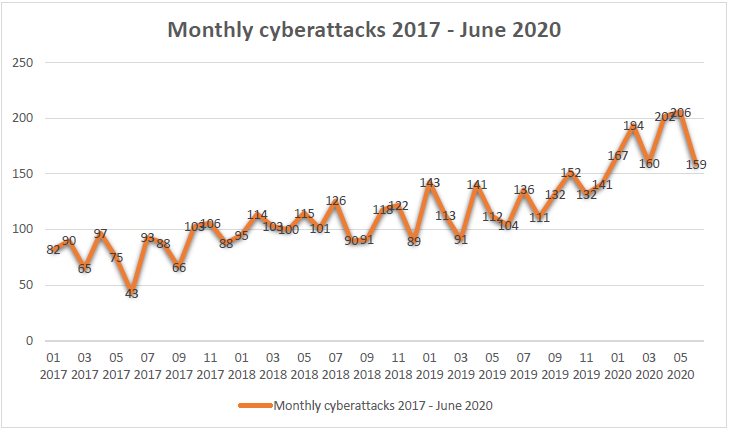
\includegraphics[width=1\textwidth]{graphics/threatscape_chart.PNG}
            \caption{Increasing number of monthly cyber attacks since 2017. Data is compiled from \cite{pt_threatscape_2018}, \cite{pt_threatscape_2019}, \cite{pt_threatscape_2020} and              \cite{pt_threatscape_2020q2}.}
            \label{fig:no_attacks_evolution}
        \end{figure}
		
	
		
	\section{Motivations}
	    \label{sec:intro_motivations}
	    
	    I chose to explore Inter Component Communication vulnerabilities on Android in this project for reasons based on the current state of mobile application security and how this vulnerability category is touched upon in related work.
	    
	    \subsection{ICC-related vulnerabilities in current mobile apps}
	    
    	One of the categories of vulnerabilities that the authors of \cite{pt_mobile_apps_2019} analysed was Inter Process Communication related vulnerabilities. Inter Process Communication, abbreviated as IPC, refers to any exchange of information between two or more running processes on a computer system. In regards to Android, \cite{pt_mobile_apps_2019} also uses the term Inter Component Communication, or ICC, interchangeably with IPC. Android components are the logical building blocks of an app, and components can communicate with other components, which can belong to the same app or to another app on the same device. Android components, especially if they are of the same app, can run in the same process. Therefore, IPC and ICC are not synonymous, even though they often overlap.
    	
    	In the study conducted in \cite{pt_mobile_apps_2019}, 29 percent of client apps used insecure inter-process communication, and the average Android app had 1.1 ICC-related vulnerabilities \cite{pt_mobile_apps_2019}.
    	
    	Insecure inter-component communication is a high-risk vulnerability, and it is more dangerous than insecure storage or transmission of data, inadequate brute force protection or other common vulnerabilities \cite{pt_mobile_apps_2019}, and therefore deserves significant attention from developers and cyber security specialists.
		
		For Phil : Should the first and second paragraph of this subsection be moved to the Current State of Cyber Security section? 
		
		Moreover, while the overwhelming majority of vulnerabilities of other types are introduced in apps through the use of third-party libraries and rarely through developer code, ICC vulnerabilities differ in this regard. According to \cite{android_vulnerabilities_evolution}, between a third and a half of ICC vulnerabilities come from code written by the developer directly. Therefore, education regarding this type of vulnerability addressed to the average developer would greatly help with minimizing the occurrence of these faults.
		
		\subsection{ICC-related vulnerabilities in related work}
		
		Vulnerabilities and cyber attacks concerning communication between Android components are not showcased in detail or intuitively in real word projects similar to mine. These projects either only cover some types of ICC related vulnerabilities, none at all, or are not easy to use, do not have good guidance, or do not show a realistic scenario.
		
		Damn Insecure and Vulnerable App has challenges 9 and 10 that show examples of hijacking intents meant for a vulnerable activity \cite{diva_walkthrough}. DIVA also contains challenge 11 where a malicious user can send intents to extract data from an unprotected content provider. 
		
		Purposefully Insecure and Vulnerable Android Application, also called PIVAA from here on, has three challenges on components that are insecurely exported and thus can be sent malicious intents. The challenges show this vulnerability in a broadcast receiver, a service and a content provider, respectively.
		
		Another intentionally insecure Android app used for educational purposes is InsecureBankv2 \cite{android_insecure_bank_github}. Similarly to PIVAA, it contains vulnerable components that can be started by a malicious app which injects a specially crafted intent, though it has a vulnerable activity, broadcast receiver and content provider and no service, unlike PIVAA \cite{android_insecure_bank_walkthrough}. Furthermore, another ICC related vulnerability it contains is intent sniffing, which allows a malware to intercept intents sent by components of the vulnerable app.
		
		Damn Vulnerable Web Application, an intentionally insecure web application with vulnerabilities such SQL injection or Cross Site Scripting, does not cover any Inter Process vulnerabilities. TryHackMe.com is an interactive website for learning cyber security and penetration testing. Although easy to use and very useful, it has no dedicated activities on IPC.
		
		None of the projects mentioned in this subsection cover all types of ICC vulnerabilities. Furthermore, DIVA, PIVAA and InsecureBankv2 only offer one application which has various components for each individual vulnerability they implement, they do not offer standalone apps for each vulnerability. More importantly, these applications are meant to be used together with other tools such as ADB or Dozer on a computer in order to perform each cyber attack. Thus, these projects do not offer real examples of malicious apps that can attack vulnerable apps. Another area in which these projects are lacking in is the educational instructions provided in the app. They provide little to no instructions, and only some hints as to how to solve each vulnerability, they do not show detailed explanations and code examples of the vulnerability and how to fix it. In addition, they do not provide much interactivity, and have to be used together with a computer. Finally, some of the apps contain major UI bugs, such as the About project activity in PIVAA.
		
		Damn Vulnerable Web Application, or DVWA, had multiple security levels for each vulnerability, where in each one the vulnerable program uses code that is increasingly secure. It tells the user what each level does, why it is not perfect, and shows source code for it. This is a very useful feature that is not shared by the three insecure Android app projects mentioned above in this subsection.
		
		\subsection{Motivation Conclusion}
		
		We have shown how vulnerabilities related to Inter Component Communication in Android are widespread and that they offer a dangerous attack surface through which applications can be hacked. Furthermore, current projects that implement intentionally insecure Android apps do not cover the domain of Inter Component Communication well and have a lot of room for improvement. 
		
		I have therefore chosen to create an educational tool that explores vulnerabilities related to insecure Inter Component Communication in Android that provides clear guidance, is interactive and combines the best parts from each of the related projects that I have looked into.
		
		For Phil: Is the above paragraph good? Is this whole Motivation section too long? Do I add personal motivations?
		
	\section{Project Aims and objectives}
		\label{sec:intro_objective} 
		
		In this section, we will discuss the causes of the precarious security of apps and why educational tools are a good solution. Following that, I will present the aim of this project, and the actions or objectives that will be undertakes to achieve said aims. 
		
		\subsection{Overview}
		
		Why is it that Android app security is often neglected? The reality is that software developers are not always trained in cybersecurity, may lack costly automatic analysis tools, or do not have the time to design and implement secure software due to tight deadlines \cite{malwarebytes_blog}. These issues can be caused by upper management not being aware of the importance of cyber security. Therefore, there needs to be more awareness of cyber security, and of vulnerabilities related to ICC in particular, in the software development industry, especially among developers, penetration testers and project managers.
		
		
	\section{Overview}  
		\label{sec:intro_overview} 
		
		The remainder of Chapter \ref{chap:intro} explains the document structure, the aims and objectives of the project, the motivations behind undertaking it and the main contributions of this piece of work.
	
	\section{Contributions} 
		\label{sec:intro_contribs} 
		
		The main contributions of this work can be seen as follows:
		
		\begin{description}	
		
			\item[$\bullet$ A LaTeX thesis template]\hfill
			
			Modify this document by adding additional TeX files for your top level content chapters. 
			
			\item[$\bullet$ A typesetting guide of useful primitive elements]\hfill
			
			Use the building blocks within this template to typeset each part of your document. Aim to use simple and reusable elements to keep your LaTeX code neat and to make your document consistently styled throughout.
			
			\item[$\bullet$ A review of how to find and cite external resources]\hfill
						
			We review techniques and resources for finding and properly citing resources from the prior academic literature and from online resources.
			
		\end{description}